\section{Колебательно-вращательные гамильтонианы в молекулярной системе координат}

При выводе молекулярного гамильтониана полиатомной системы часто предполагается, что амплитуда колебаний мала. Гамильтониан, полученный Вильсоном и Говардом, для системы с колебаниями малой амплитуды широко используется и часто служит базисом для дальнейших уточнений. \par
Однако колебания большой амплитуды, проявляющиеся в в слабосвязанных комплексах не могут быть описаны при помощи того же подхода. Для описания колебаний большой амплитуды часто используются координаты Якоби, координаты Радау, гиперсферические координаты и др. \par 
Координаты Якоби являются обобщением координат, использованных нами в двухатомной системе, на случай системы $N$ тел \cite{greiner, littlejohn1995}. Рассмотрим систему из $N$ частиц с массами $\lb m_1, \dots m_N \rb$ и координатами $\lb \mf{r}_1, \dots, \mf{r}_N \rb$ в лабораторной системе координат. Лагранжева кинетическая энергия в лабораторной системе координат записывается как
\begin{gather}
    T_\text{tot} = \frac{1}{2} \sum_{k = 1}^N m_k \dot{\mf{r}}_k^2.
\end{gather}

Чтобы отделить трансляционные степени свободы произведем линейную замену координат  $\lb \mf{r}_1 \dots \mf{r}_N \rb \rightarrow \lb \bs{\rho}_1, \dots \bs{\rho}_{N} \rb$: 
\begin{gather}  
    \lc
    \begin{aligned}
        \bs{\rho}_1 &= \frac{m_1 \mf{r}_1}{m_1} - \mf{r}_2 = \mf{r}_1 - \mf{r}_2, \\
        \bs{\rho}_2 &= \frac{m_1 \mf{r}_1 + m_2 \mf{r}_2}{m_1 + m_2}, \\
        \mf{\rho}_j &= \frac{\displaystyle \sum_{k = 1}^j m_k \mf{r}_k}{\displaystyle \sum_{k = 1}^j m_k} - \mf{r}_{j + 1}, \quad 2 < j < N \\
        \mf{\rho}_N &= \frac{1}{M} \sum_{k = 1}^N m_k \mf{r}_k,
    \end{aligned}
    \right.
\end{gather}
%
где через $M$ обозначена суммарная масса системы частицы. \par
Первый вектор Якоби $\bs{\rho}_1$ соединяет частицы 1 и 2. Второй вектор Якоби соединяет центр масс первых двух частиц и третью частицу. Третий вектор Якоби соеднияет центр масс первых трех частиц и четвертую частицу и т.д. Последний вектор Якоби суть вектор, направленный в центр масс системы. Пример векторов Якоби для системы, соcтоящей из трех частиц, приведен на Рис. \ref{fig:jacobi_coordinates}. 

\begin{figure}
    \centering
    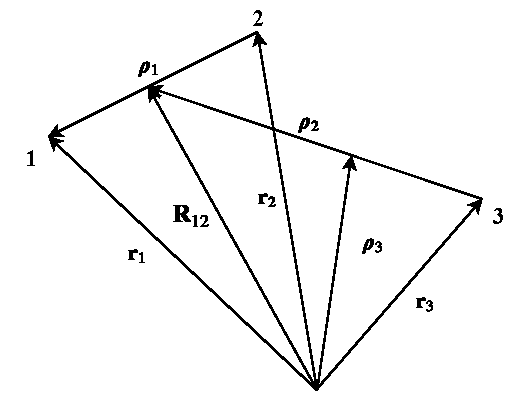
\includegraphics[width=0.5\linewidth]{pictures/jacobi_coordinates.pdf}
    \caption{Координаты Якоби  для системы из 3 частиц, пронумерованных 1, 2, 3. Через $\mf{R}_{12}$ бозначен вектор, направленный в центр масс пары частиц 1 и 2.}
    \label{fig:jacobi_coordinates}
\end{figure}

Можно показать, что кинетическая энергия в лагранжевой форме, выраженная через векторы Якоби записывается как \cite{greiner} 
\begin{gather}
    T_\text{tot} = \frac{1}{2} M \dot{\bs{\rho}}_N^2 + \frac{1}{2} \sum_{k = 1}^{N - 1} \mu_k \dot{\bs{\rho}}_k^2,
\end{gather}
%
где приведенные массы $\mu_j$ связаны с исходными массами $m_j$ следующими соотношениями
\begin{gather}
    \frac{1}{\mu_j} = \frac{1}{M_j} + \frac{1}{m_{j+1}}, \quad M_j = \sum_{k = 1}^j m_k, \quad j = 1 \dots N - 1. \label{polyatom-jacobi-masses}
\end{gather}

Отделяя центр масс, мы приходим к следующей форме кинетической энергии
\begin{gather}
    \Tl = \frac{1}{2} \sum_{k = 1}^{N - 1} \mu_k \dot{\bs{\rho}}_k^2.
\end{gather}

Для отделения вращательных степеней свободы введем подвижную систему координат. Лабораторная и подвижная системы координат связаны друг с другом матрицей ортогонального преобразования $\bbS$ \cite{goldstein}. Обозначим через $\mf{R}_j$ координаты векторов Якоби в подвижной системе координат. Введенные векторы $\mf{R}_j$ связаны с векторами в лабораторной системе линейным преобразованием
\begin{gather}
    \boldsymbol{\rho}_j = \bbS \mf{R}_j.
\end{gather}
Будем рассматривать параметризацию матрицы ортогонального преобразования $\bbS$ тройкой углов Эйлера $\Phi$, $\Theta$, $\Psi$ \cite{goldstein}
\begin{gather}
    \bbS = 
    \begin{bmatrix}
        \cos \Psi \cos \Phi - \cos \Theta \sin \Phi \sin \Psi & -\sin \Psi \cos \Phi - \cos \Theta \sin \Phi \cos \Psi & \sin \Theta \sin \Phi \\ 
        \cos \Psi \sin \Phi + \cos \Theta \cos \Phi \sin \Psi & -\sin \Psi \sin \Phi + \cos \Theta \cos \Phi \cos \Psi & - \sin \Theta \cos \Phi \\
        \sin \Theta \sin \Psi & \sin \Theta \cos \Psi & \cos \Theta
    \end{bmatrix}.
\end{gather}

Лагранжева кинетическая энергия в подвижной системе отсчета может быть записана как \cite{landau-volume1}
\begin{gather}
    \Tl = \frac{1}{2} \sum_{i = 1}^{N-1} \mu_i \dot{\mf{R}}_i^2 + \frac{1}{2} \sum_{i = 1}^{N - 1} \mu_i \lsq \boldsymbol{\Omega} \times \mf{R}_i \rsq^2 + \boldsymbol{\Omega}^{+} \sum_{i = 1}^{N - 1} \mu_i \lsq \mf{R}_i \times \dot{\mf{R}}_i \rsq,
\end{gather}
%
где $\boldsymbol{\Omega}$ -- вектор угловой скорости в проекции на подвижную систему координат. Вектор угловой скорости $\boldsymbol{\Omega}$ связан с углами Эйлера и эйлеровыми скоростями следующим соотношением
\begin{gather}
    \boldsymbol{\Omega} = \bbV \mf{v} = 
    \begin{bmatrix}
        \sin \Theta \sin \Psi & \cos \Psi & 0 \\
        \sin \Theta \cos \Psi & -\sin \Psi & 0 \\
        \cos \Theta & 0 & 1 
    \end{bmatrix}
    \begin{bmatrix}
        \dot{\Phi} \\ \dot{\Theta} \\ \dot{\Psi}
    \end{bmatrix}.
\end{gather}

Введем набор внутренних координат $\mf{q} = \lb q_1, \dots q_s \rb$ и, используя связь координат Якоби с введенными координатами $\mf{R}_j = \mf{R}_j(\mf{q})$, перепишем выражение для кинетической энергии в форме \cite{petrov2015}
\begin{gather}
    \Tl = \frac{1}{2} \dot{\mf{q}}^+ \bba \dot{\mf{q}} + \bOmega^+ \bbA \mf{q} + \frac{1}{2} \bOmega^+ \bbI \, \bOmega, \label{body-fixed-lagrange-energy} 
\end{gather}
%
где через $\bba, \bbA, \bbI$ обозначены матрица относительной кинетической энергии, кориолисова матрица и матрица тензора инерции, соответственно. Элементы матриц относительной кинетической энергии и кориолисова взаимодействия заданы следующими выражениями
\begin{gather}
    \bba_{jk} = \sum_{i = 1}^{N - 1} \mu_i \frac{\partial \mf{R}_i}{\partial q_j} \frac{\partial \mf{R}_i}{\partial q_k}, \quad \bbA_{jk} = \sum_{i = 1}^{N - 1} \mu_i \lsq \mf{R}_i \times \frac{\partial \mf{R}_i}{\partial q_k} \rsq_j. \label{polyatom-kinetic-energy-matrices}
\end{gather}

Выражение для кинетической энергии \eqref{body-fixed-lagrange-energy} для перехода к Гамильтоновой форме удобно переписать в матричном виде
\begin{gather}
    \Tl = \frac{1}{2} \begin{bmatrix} \bOmega^+ & \dot{\mf{q}}^+ \end{bmatrix} \bbB \begin{bmatrix} \bOmega \\ \dot{\mf{q}} \end{bmatrix}, \label{polyatom-block-matrix-kin-energy}
\end{gather}
%
где через $\bbB$ обозначена блочная матрица со следующими элементами 
\begin{gather}
    \bbB = \begin{bmatrix} 
    \bbI & \bbA \\ \bbA^+ & \bba 
    \end{bmatrix}.
\end{gather}

Можно показать, что если ввести величину $\mf{J}$ как производную кинетической энергии в лагранжевой форме $\Tl$ по вектору угловой скорости $\bOmega$, то $\mf{J}$ суть вектор углового момента в подвижной системе координат (приложение \ref{appendix:angular-momentum-body-fixed}). Обобщенные импульсы $\mf{p}$, сопряженные координатам $\mf{q}$, по определению ранвы производным кинетической энергии в лагранжевой форме $\Tl$ по обобщенным скоростям $\dot{\mf{q}}$: 
\begin{gather}
    \mf{J} = \frac{\partial \Tl}{\partial \bOmega} = \bbI \bOmega + \bbA \dot{\mf{q}}, \label{polyatom-angmom1} \\
\mf{p} = \frac{\partial \Tl}{\partial \dot{\mf{q}}} = \bbA^+ \bOmega + \bba \dot{\mf{q}} \label{polyatom-gen-momenta}.
\end{gather}

Заметим, что выражения \eqref{polyatom-angmom1}, \eqref{polyatom-gen-momenta} могли быть получены дифференцированием выражения  \eqref{polyatom-block-matrix-kin-energy} по блочному вектору с компонентами $\bOmega$ и $\dot{\mf{q}}$. Выражения для углового момента и обобщенных импульсов объединим в один блочный вектор
\begin{gather}
    \begin{bmatrix} \mf{J} \\ \mf{p} \end{bmatrix} = \bbB \begin{bmatrix} \bOmega \\ \dot{\mf{q}} \end{bmatrix} = 
    \begin{bmatrix} \bbI & \bbA \\ \bbA^+ & \bba \end{bmatrix} \begin{bmatrix} \bOmega \\ \dot{\mf{q}} \end{bmatrix}.
\end{gather}

Для того, чтобы выразить лагранжевы переменные из полученного выражения, нам необходимо обратить блочную матрицу $\bbB$. Это обращение удобно выполнить при помощи формул Фробениуса \cite{petrov2015, gantmaher}. Через $\bbG$ обозначают обратную матрицу к $\bbB$, ее матричные компоненты выражаются как
\begin{gather}
    \begin{aligned}
        \bbG_{11} &= \lb \bbI - \bbA \bba^{-1} \bbA^+ \rb^{-1} \\
        \bbG_{12} &= -\bbI^{-1} \bbA \bbG_{22} = -\bbG_{11} \bbA \bba^{-1} \\
        \bbG_{21} &= -\bba^{-1} \bbA^+ \bbG_{11} = \bbG_{22} \bbA^+ \bbI^{-1} \\
        \bbG_{22} &= \lb \bba - \bbA^+ \bbI^{-1} \bbA \rb^{-1}
    \end{aligned} \label{polyatom-frobenius}
\end{gather}

Переход от кинетической энергии в форме Лагранжа к кинетической энергии в форме Гамильтона осуществляем при помощи стандартной процедуры \cite{goldstein}
\begin{gather}
    \Th = \begin{bmatrix} \bOmega^+ & \dot{\mf{q}}^+ \end{bmatrix} \begin{bmatrix} \mf{J} \\ \mf{p} \end{bmatrix} - \Tl = \frac{1}{2} \begin{bmatrix} \mf{J}^+ & \mf{p}^+ \end{bmatrix} \bbG \begin{bmatrix} \mf{J} \\ \mf{p} \end{bmatrix} = \frac{1}{2} \mf{J}^+ \bbG_{11} \mf{J} + \mf{J}^+ \bbG_{12} \mf{p} + \frac{1}{2} \mf{p}^+ \bbG_{22} \mf{p}. 
\end{gather}

В этой работе мы будем работать только с системами, состоящими из жесткой линейной молекулы и атома и из двух жестких линейных молекул. В первом случае зададим подвижную систему координат таким образом, чтобы два вектора Якоби лежали в плоскости подвижной системы $OXZ$, причем дополнительно потребуем, чтобы вектор $\mf{R}_2$, соединяющий центр масс линейной молекулы с атомом, лежал вдоль оси $OZ$ (см. рис. \ref{fig:body-fixed-linear-atom}). Такое определение системы координат известно как $R$-вложение \cite{tennyson1986}. Обозначим длину линейной молекулы через $l$.
    
\begin{figure}[H]
    \centering
    %\begin{minipage}{0.49\linewidth}
    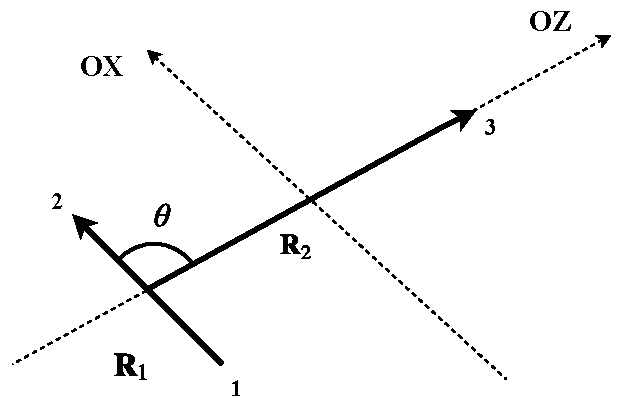
\includegraphics[width=0.5\linewidth]{pictures/triatom_coordinates.pdf}
    %\end{minipage}
    %\begin{minipage}{0.49\linewidth}
    %    Взять картинку из будущей статьи с N$_2$-N$_2$
    %\end{minipage}
    \caption{Молекулярная система координат для системы линейная молекула-атом}
    \label{fig:body-fixed-linear-atom}
\end{figure}

В качестве обобщенных координат выберем $R$ -- длину вектора Якоби $\mf{R}_2$ или, что эквивалентно, расстояние от атома до центра масс линейной молекулы, и угол $\theta$ между векторами Якоби $\mf{R}_1$ и $\mf{R}_2$. Выпишем соотношения между обобщенными координатами $\mf{q}$ и координатами векторов Якоби в подвижной плоскости
\begin{gather}
    \begin{aligned}
        X_1 &= l \sin \theta \\
        Y_1 &= 0 \\
        Z_1 &= l \cos \theta
    \end{aligned} \qquad
    \begin{aligned}
        X_2 &= 0 \\ 
        Y_2 &= 0 \\
        Z_2 &= R 
    \end{aligned}. \label{linear-molecule-atom-jacobi-coords}
\end{gather}

Вывод дальнейших выражений реализовывался в системе компьютерной алгебры Maple. Координаты векторов Якоби \eqref{linear-molecule-atom-jacobi-coords} использовались для расчета компонент матриц относительной кинетической энергии, кориолисова взаимодействия и тензора инерции по выражениям \eqref{polyatom-kinetic-energy-matrices}. В случае линейная молекула$-$атом блоки матрицы $\bbG$ могут быть получены в компактном виде. Уже для случая двух жестких линейных молекул выражения для блоков матрицы $\bbG$ оказываются слишком громоздкими, поэтому была разработана схема реализации траекторного расчета, избегающая аналитической работы с компонентами этих матриц, переносимая на системы с произвольным количеством вращательных степеней свободы. \par
В качестве примера системы линейная молекула$-$атом мы выбрали CO$_2-$Ar. Внутримолекулярные колебания молекулы CO$_2$ происходят существенно быстрее межмолекулярных движений комплекса с атомом аргона, поэтому предполагается, что взаимодействие между внутри- и межмолекулярными колебательными модами в данном случае компенсируется. Приведенные массы частиц Якоби согласно \eqref{polyatom-jacobi-masses} равны
\begin{gather}
    \mu_1 = \frac{m_1}{2}, \quad \mu_2 = \frac{m_2 \lb 2 m_1 + m_3 \rb}{2 m_1 + m_2 + m_3},
\end{gather}
% 
где через $m_1$ обозначена масса атома кислорода, через $m_2$ -- масса атома аргона, через $m_3$ -- масса атома углерода. \par
При помощи системы компьютерной алгебры были получены следующие выражения для матриц кинетической энергии в форме Лагранжа
\begin{gather}
	\bba =
	\begin{bmatrix}
		\mu_2 & 0 \\
		0 & \mu_1 l^2
	\end{bmatrix}, \quad 
	\bbA = 
	\begin{bmatrix}
		0 & 0 \\
		0 & \mu_1 l^2 \\
		0 & 0 
	\end{bmatrix}, \quad
	\bbI = 
	\begin{bmatrix}
		\mu_1 l^2 \cos^2 \theta + \mu_2 R^2 & 0 & -\mu_1 l^2 \sin \theta \cos \theta \\
		0 & \mu_1 l^2 + \mu_2 R^2 & 0 \\
		- \mu_1 l^2 \sin \theta \cos \theta & 0 & \mu_1 l^2 \sin^2 \theta
	\end{bmatrix}. \notag
\end{gather}

Подставив полученные выражения для матриц в формулы Фробениуса \eqref{polyatom-frobenius}, приходим к следующим выражениям для матриц, определяющим кинетическую энергию в форме Гамильтона 
\begin{gather}
	\bbG_{11} =
	\begin{bmatrix}
		\dfrac{1}{\mu_2 R^2} & 0 & \dfrac{\ctg \theta}{\mu_2 R^2} \\
		0 & \dfrac{1}{\mu_2 R^2} & 0 \\
		\dfrac{\ctg \theta}{\mu_2 R^2} & 0 & \dfrac{\ctg^2 \theta}{\mu_2 R^2} + \dfrac{1}{\mu_1 l^2 \sin^2 \theta}
	\end{bmatrix}, \quad
	\bbG_{12} =
	\begin{bmatrix}
		0 & 0 \\
		0 & - \dfrac{1}{\mu_2 R^2} \\
		0 & 0
	\end{bmatrix}, \quad 
	\bbG_{22} = 
	\begin{bmatrix}
		\dfrac{1}{\mu_2} & 0 \\
		0 & \dfrac{1}{\mu_2 R^2} + \dfrac{1}{\mu_1 l^2}
	\end{bmatrix}. \notag
\end{gather}

Итак, кинетическая энергия в форме Гамильтона для системы CO$_2-$Ar в выбранной нами молекулярной системе отсчета получается следующей
\begin{gather}
\Th = \frac{1}{2 \mu_2} p_R^2 + \lb \frac{1}{2 \mu_2 R^2} + \frac{1}{2 \mu_1 l^2} \rb p_\theta^2 - \frac{1}{\mu_2 R^2} p_\theta \Jy + \frac{1}{2 \mu_2 R^2} \Jy^2 + \frac{1}{2 \mu_2 R^2} \Jx^2 + \frac{1}{2 \sin^2 \theta} \lb \frac{\cos^2 \theta}{\mu_2 R^2} + \frac{1}{\mu_1 l^2} \rb \Jz^2 + \notag \\
+ \frac{\ctg \theta}{\mu_2 R^2} \Jx \Jz. 
\end{gather}



\begin{subappendices}
    \section{Вектор углового момента в подвижной системе отсчета} \label{appendix:angular-momentum-body-fixed}

    Рассмотрим производную кинетической энергии в лагранжевой форме $\Tl$ по вектору угловой скорости $\bOmega$, компонентны которого выражены в подвижной системе отсчета. Продифференцировав выражение \eqref{body-fixed-lagrange-energy} по вектору угловой скорости, получаем 
    \begin{gather}
        \frac{\partial \Tl}{\partial \bOmega} = \bbA \dot{\mf{q}} + \bbI \bOmega. \label{appendix-angular-momentum1}
    \end{gather}

    Несложно показать, что вектор углового момента $\mf{j}$ в лабораторной системе отсчета может быть записан через векторы Якоби как
    \begin{gather}
        \mf{j} = \sum_{i = 1}^{N - 1} \mu_i \lsq \bs{\rho}_i \times \dot{\bs{\rho}}_i \rsq. \label{appendix-angular-momentum-jacobi-vectors}
    \end{gather}

    Выразим производная вектора $\bs{\rho}_i$ в лабораторной системе координат через производную в подвижной системе координат \cite{goldstein}
    \begin{gather}
        \dot{\bs{\rho}}_i = \bbS \lb \dot{\mf{R}}_i + \lsq \bs{\Omega} \times \mf{R}_i \rsq \rb. \label{appendix-jacobi-vector-derivative} 
    \end{gather}

    Подставив выражение \eqref{appendix-jacobi-vector-derivative} в выражение углового момента \eqref{appendix-angular-momentum-jacobi-vectors} и осуществив несложные алгебраические преобразования, приходим к 
    \begin{gather}
        \mf{j} = \sum_{i = 1}^{N-1} \mu_i \lsq \bs{\rho}_i \times \bbS \lb \dot{\mf{R}}_i + \Big[ \bOmega \times \mf{R}_i \Big] \rb \rsq = \bbS \sum_{i = 1}^{N-1} \mu_i \Big[ \mf{R}_i \times \dot{\mf{R}}_i \Big] + \bbS \sum_{i = 1}^{N-1} \mu_i \Big[ \mf{R}_i \times \lsq \bOmega \times \mf{R}_i \rsq \Big] = \bbS \bbA \dot{\mf{q}} + \bbS \bbI \bOmega.
    \end{gather}

    Умножая обе части на матрицу $\bbS^{-1}$, получаем в правой части выражение \eqref{appendix-angular-momentum1}
    \begin{gather}
        \bbS^{-1} \mf{j} = \bbA \dot{\mf{q}} + \bbI \bOmega.
    \end{gather}

    Согласно введенному определению матрицы $\bbS$, выражение в левой части суть вектор углового момента в подвижной системе отсчета. Таким образом, мы показали, что производная кинетической энергии в лагранжевой форме по вектору угловой скорости в подвижной системе равна вектору углового момента в подвижной системе
    \begin{gather}
        \mf{J} = \frac{\partial \Tl}{\partial \bOmega}.
    \end{gather}
    
\end{subappendices}
